\documentclass[conference]{IEEEtran}
\IEEEoverridecommandlockouts

\usepackage{cite}
\usepackage{amsmath,amssymb}
\usepackage{graphicx}
\usepackage{booktabs}
\usepackage{multirow}
\usepackage{array}
\usepackage{xcolor}
\usepackage{url}
\usepackage[hidelinks]{hyperref}

\graphicspath{{figures/}}

% The headline numbers (macros in results_macros.tex) and every table body
% (tab_*.tex) are regenerated from the notebook's result tables by make_macros.py.
% Secondary numbers quoted in the prose of Sections IV and V are typed by hand from
% the same tables and must be re-checked if the notebook is re-run.
% Generated by make_macros.py -- do not edit by hand.
% Source: master_thesis_on_churn_prediction | quick_run = False
\newcommand{\NRows}{1,000,000}
\newcommand{\NCols}{32}
\newcommand{\NTrain}{800,000}
\newcommand{\NTest}{200,000}
\newcommand{\NDev}{200,000}
\newcommand{\NTune}{100,000}
\newcommand{\ChurnRatePct}{9.92}
\newcommand{\ImbRatio}{9.1}
\newcommand{\NEngineered}{Twenty-four}
\newcommand{\NBaseline}{29}
\newcommand{\NEngSet}{52}
\newcommand{\McDraws}{20,000}
\newcommand{\CampaignSharePct}{2}
\newcommand{\ChampionLong}{logistic regression at default settings on the raw features}
\newcommand{\ChampionShort}{LR}
\newcommand{\BestDlShort}{ANN}
\newcommand{\ChampAucTest}{0.6848}
\newcommand{\BestDlAucTest}{0.6851}
\newcommand{\TestAucMin}{0.671}
\newcommand{\TestAucMax}{0.685}
\newcommand{\TestSpread}{0.014}
\newcommand{\TrainRatioBestDl}{50}
\newcommand{\ChampOnlineMs}{2.0}
\newcommand{\BestDlOnlineMs}{5.5}
\newcommand{\GpuSlowdownDnn}{5.3}
\newcommand{\GpuSlowdownAnn}{8.1}
\newcommand{\HwChip}{Apple M1}
\newcommand{\HwCores}{8}
\newcommand{\HwRam}{16}
\newcommand{\HwOs}{macOS 27.0}
\newcommand{\TfVersion}{2.16.2}
\newcommand{\MetalVersion}{1.2.0}
\newcommand{\SkVersion}{1.8.0}
\newcommand{\XgbVersion}{3.2.0}
\newcommand{\OptunaVersion}{4.8.0}
\newcommand{\ShapVersion}{0.46.0}

\newcommand{\LitPoolN}{351}
\newcommand{\LitAbstractN}{338}
\newcommand{\LitBankN}{53}
\newcommand{\LitAllN}{338}
\newcommand{\LitBothN}{69}
\newcommand{\LitBothTimeN}{9}
\newcommand{\LitBothTimeStatN}{one}
\newcommand{\LitBankBothN}{7}
\newcommand{\LitBankMl}{66}
\newcommand{\LitAllMl}{67}
\newcommand{\LitBankDl}{32}
\newcommand{\LitAllDl}{34}
\newcommand{\LitBankAcc}{72}
\newcommand{\LitAllAcc}{64}
\newcommand{\LitBankAuc}{21}
\newcommand{\LitAllAuc}{21}
\newcommand{\LitBankTime}{13}
\newcommand{\LitAllTime}{9}
\newcommand{\LitBankStat}{2}
\newcommand{\LitAllStat}{1}
\newcommand{\LitBankImb}{28}
\newcommand{\LitAllImb}{23}
\newcommand{\LitBankXai}{25}
\newcommand{\LitAllXai}{18}
\newcommand{\LitBankHpo}{21}
\newcommand{\LitAllHpo}{12}
\newcommand{\LitBankBoth}{13}
\newcommand{\LitAllBoth}{20}


\newcommand{\rev}[1]{#1}

\begin{document}

\title{Machine Learning versus Deep Learning for Customer Churn Prediction: A Leakage-Controlled Head-to-Head on One Million Customers}

\author{\IEEEauthorblockN{Duc Le}
\IEEEauthorblockA{% TODO(author): department, institution, city, country, and contact e-mail
\textit{Affiliation to be completed}}}

\maketitle

\begin{abstract}
Deep learning is often reported to outperform classical machine learning for customer churn prediction, yet the supporting studies rarely place both families under one protocol, test whether differences are real, or measure serving cost. We report a controlled head-to-head of four machine-learning models (logistic regression, decision tree, random forest, XGBoost) and two feed-forward networks on \NRows{} customer records with a \ChurnRatePct\% churn rate. All preprocessing and resampling is confined to training folds; staged experiments separate feature engineering from tuning; four imbalance treatments and three search strategies are compared on shared folds; and differences are judged with paired tests, Holm correction and a pre-declared materiality threshold. On \NTest{} held-out customers the six models span only \TestSpread{} ROC-AUC (\TestAucMin{}--\TestAucMax{}). The selected model, \ChampionLong{}, scores \ChampAucTest{} against \BestDlAucTest{} for the best default network, while training \TrainRatioBestDl{} times faster and answering a request in \ChampOnlineMs{}~ms against \BestDlOnlineMs{}~ms. A 50-trial search over the networks' depth, width, activation and regularisation selected a small network with a direct linear path that matched logistic regression (cross-validated difference $+0.0002$, $p=0.36$; test ROC-AUC 0.6846) and did not exceed it. On the GPU the networks trained \GpuSlowdownDnn{} times slower than on the CPU. Six falsifiable tests explain the outcome: the log-odds are close to linear and additive, so there is no interaction structure for a network to exploit. A Monte Carlo campaign simulation shows that neither the accuracy gap nor the compute bill decides the choice; the case against deep learning by default rests on training time, latency under load, data requirements and explainability. Deep learning should be adopted for churn scoring only when a like-for-like test shows a material gain.
\end{abstract}

\begin{IEEEkeywords}
customer churn, banking, deep learning, gradient boosting, class imbalance, hyperparameter optimisation, data leakage, SHAP, inference latency, Monte Carlo simulation
\end{IEEEkeywords}

% =============================================================================
\section{Introduction}
% =============================================================================
Retaining a customer is cheaper than acquiring one, so banks invest in models that rank customers by their risk of leaving and direct a limited retention budget to the top of that ranking~\cite{verbeke2012new,manzoor2024review}. The modelling question has become a choice between two families. Classical machine learning (ML), in particular tree ensembles, is fast and comparatively transparent. Deep learning (DL) promises to learn feature interactions automatically, and a growing share of banking studies report that it wins: a deep network was the most accurate model at the Commercial Bank of Ethiopia~\cite{seid2022machine}, a recurrent architecture was reported as significantly superior to traditional techniques on Iranian banking data~\cite{haddadi2022iranian}, and artificial neural networks have been reported at 86--87\% accuracy on the public bank churn benchmark~\cite{zaky2022banking,baby2023artificial}.

A practitioner cannot act on these reports, for three reasons. First, the two families are seldom evaluated under one protocol: the preprocessing, the imbalance treatment, the tuning effort and the data split differ between the models being compared, so a reported gap cannot be attributed to the model. Second, the headline metric is usually accuracy, which a model that predicts ``no churn'' for everyone already maximises on imbalanced data~\cite{raj2023machine}. Third, the cost of the model in production, namely its training time, its latency per request and what it takes to explain a decision to a regulator, is rarely measured, although it is what a bank pays for every month.

This paper addresses the question directly: \emph{given that deep learning is known for strong predictive performance, should it be the default choice for production churn scoring, and if not, why not?} We answer it with a single experimental pipeline in which the only thing that differs between the six models is the model. The contributions are as follows.
\begin{enumerate}
\item \textbf{A like-for-like protocol.} Six models share the same folds, seeds, preprocessing graph, metrics and timing protocol, and all fitted statistics and all resampling are confined to training folds. We measure what the common alternative, resampling before splitting, would have reported.
\item \textbf{Attribution of gains.} Three staged experiments isolate the effect of feature engineering and of hyperparameter tuning, and an ablation isolates the effect of four imbalance treatments on both model families.
\item \textbf{Significance and materiality.} Paired tests with multiplicity correction are reported alongside a materiality threshold declared before the results were seen, so that reliable but negligible differences are identified as such.
\item \textbf{Execution cost as a first-class result.} Training time, batch and single-request latency, behaviour under concurrent load, and a CPU-versus-GPU benchmark are measured under one protocol.
\item \textbf{An explanation of the outcome.} Six falsifiable tests diagnose why the ranking came out as it did, and a Monte Carlo simulation converts the accuracy and latency differences into campaign value.
\end{enumerate}

% =============================================================================
\section{Research Problem and Literature Review}
% =============================================================================
\subsection{Scope of the review}
We queried Crossref for IEEE-published work (DOI prefix 10.1109, 2015--2026) with 24 search strings covering churn prediction in banking, telecommunications, e-commerce, insurance and subscription services, and the methodological themes of imbalance, tuning, explainability and deep learning on tabular data. After removing records unrelated to customer churn, \LitPoolN{} papers remained; abstracts were available for \LitAbstractN{} of them. Sixty-two papers were read in detail and are cited below; the full set was additionally screened by keyword to quantify what the literature reports (Table~\ref{tab:lit}). The screening is at abstract level and therefore understates what full texts contain; it is used to show proportions, not to make claims about individual papers.

\begin{table}[t]
\caption{What IEEE-published churn studies report, 2015--2026 (abstract-level keyword screening)}
\label{tab:lit}
\centering
\begin{tabular}{@{}lrr@{}}
\toprule
Abstract mentions & Banking & All sectors \\
 & ($n=\LitBankN$) & ($n=\LitAllN$) \\
\midrule
Classical ML model & \LitBankMl\% & \LitAllMl\% \\
Neural or deep model & \LitBankDl\% & \LitAllDl\% \\
\quad both families & \LitBankBoth\% & \LitAllBoth\% \\
Accuracy & \LitBankAcc\% & \LitAllAcc\% \\
ROC-AUC & \LitBankAuc\% & \LitAllAuc\% \\
Imbalance treatment & \LitBankImb\% & \LitAllImb\% \\
Hyperparameter optimisation & \LitBankHpo\% & \LitAllHpo\% \\
Explainability (SHAP, LIME) & \LitBankXai\% & \LitAllXai\% \\
Execution time or latency & \LitBankTime\% & \LitAllTime\% \\
Statistical significance test & \LitBankStat\% & \LitAllStat\% \\
\bottomrule
\end{tabular}
\end{table}

\subsection{Classical machine learning}
Banking studies have converged on tree ensembles. Random forest was the most accurate of four classifiers on the public bank benchmark once the minority class was oversampled~\cite{rahman2020machine}, and comparisons of logistic regression, decision trees, nearest neighbours and forests on bank data reach similar conclusions~\cite{kaur2020banking,karvana2019data,sen2015modelling}. Stacking and voting ensembles add small gains at about 87\% accuracy on a 10,000-row dataset~\cite{galal2022enhancing,galal2024enhancing}, and boosted trees tuned by metaheuristics have been applied to credit-card and bank churn~\cite{jovanovic2023credit,ponnusamy2023psosvm,gajula2025intelligent}. A systematic review of telecommunications and banking identifies ensembles, and XGBoost~\cite{chen2016xgboost} in particular, as the prevailing choice~\cite{altairey2024telecommunication}. The same pattern holds outside banking: forests and boosting lead in telecommunications~\cite{ullah2019random,mishra2017comparative,dalvi2016telecom,brandusoiu2016methods,karamollaoglu2021machine,ahmed2017review}, e-commerce~\cite{raeisi2020ecommerce,berger2019user}, insurance~\cite{he2020machine,sundarkumar2015oneclass} and subscription services~\cite{vadakattu2015enterprise,kuramannagari2025comparative}.

\subsection{Deep learning}
Neural models are the main challenger. In banking, feed-forward networks~\cite{zaky2022banking,baby2023artificial,santoso2024artificial,setiana2025improving}, deep networks~\cite{seid2022machine}, recurrent models~\cite{haddadi2022iranian,latheef2021lstm}, hybrids~\cite{hemalatha2019hybrid,pathan2026intelligent} and real-time architectures~\cite{gera2026forecasting} have all been reported as competitive or superior. Telecommunications studies report a multilayer perceptron at 94.19\% accuracy against 87.52\% for logistic regression~\cite{bharadwaj2018mobile}, a convolutional network at 98.85\%~\cite{karanovic2018telecommunication}, and purpose-built architectures above 95\% on three benchmarks~\cite{saha2024churnnet}; recurrent and behavioural models are reported to outperform their baselines~\cite{hu2018prnn,agrawal2018modelling,cao2019deep,zhang2017deep}, and hybrids feed tree outputs into a perceptron~\cite{tang2020xgboost}. A recent review recommends both ensembles and deep learning to practitioners~\cite{manzoor2024review}.

The broader evidence on tabular data points the other way. A survey of deep networks for tabular data concludes that gradient-boosted trees still mostly outperform them on supervised tasks~\cite{borisov2024deep}, a finding repeated in controlled benchmarks~\cite{grinsztajn2022tree,shwartzziv2022tabular,pasaribu2024tabular}. The churn literature and the tabular-learning literature therefore disagree, and the disagreement is what a head-to-head must resolve.

\subsection{Imbalance, tuning, explainability and metrics}
Churners are a minority, and oversampling is the standard response. SMOTE~\cite{chawla2002smote} and its variants are compared in~\cite{amin2016comparing,imani2024impact,mansoor2023banking,wu2016ecommerce}; sampling is combined with stacking in~\cite{de2022samplingbased}; and under- and oversampling are shown to trade specificity against sensitivity rather than to improve both~\cite{shumaly2020handling}. Cost-sensitive learning is the algorithm-level alternative~\cite{xiao2018costsensitive,zouaghia2026costsensitive}. GAN-based oversampling~\cite{xu2019ctgan} is rare: it appears in about 1\% of the screened abstracts. Hyperparameter optimisation is reported by Bayesian~\cite{kim2018bayesian,an2025novel} and metaheuristic~\cite{jovanovic2023credit,ponnusamy2023psosvm} search, usually with one strategy and without comparison to random search~\cite{bergstra2012random} or to a modern framework such as Optuna~\cite{akiba2019optuna}. Explainability has grown quickly, almost always through SHAP~\cite{lundberg2017unified}, in banking~\cite{raut2025bank,sarkar2026bank,zouaghia2026costsensitive,setiana2025improving} and elsewhere~\cite{leung2021explainable,ou2023interpretable,jm2025realtime}, motivated by the transparency expected of financial institutions. On metrics, accuracy remains the headline figure despite repeated warnings that it is insufficient on imbalanced data~\cite{raj2023machine,cao2019deep}; profit-based evaluation has been proposed as the measure a business actually needs~\cite{verbeke2012new,stripling2015profit,zhang2018novel}; and one data-centric study concludes that cleaning data and engineering features improves churn detection more than changing the algorithm~\cite{chowdhury2026datacentric}.

\subsection{The gap}
Table~\ref{tab:lit} quantifies three omissions. First, only \LitAllBoth\% of the screened abstracts (\LitBankBoth\% in banking) evaluate both families in one study, so most claims that one family beats the other are comparisons across papers with different data and protocols. Second, \LitAllTime\% mention execution time or latency in any form, and \LitAllStat\% mention a statistical test; among the \LitBothN{} studies that include both families, \LitBothTimeStatN{} mentions both. The practice recommended for comparing classifiers~\cite{demsar2006statistical} has not reached this literature. Third, the placement of resampling relative to the split is rarely stated, although resampling before splitting lets synthetic points derived from validation rows enter training, a recognised form of leakage~\cite{kaufman2012leakage} that inflates exactly the results that favour complex models.

There is therefore a clear demand for a head-to-head comparison of ML and DL for banking churn that (i) holds everything but the model constant, (ii) tests differences for significance and for materiality, and (iii) measures the production cost that determines whether a more accurate model is worth deploying. The answer to whether deep learning should always be used in production depends on all three, and the existing literature supplies none of them together.

% =============================================================================
\section{Methodology}
% =============================================================================
The complete pipeline is one Jupyter notebook that runs end to end from the raw file; all random seeds are fixed at 42. The network tuning study (Section~\ref{sec:nettune}) is a separate script that reuses the notebook's definitions, partitions and folds. Fig.~\ref{fig:pipeline} summarises the design.

\begin{figure}[t]
\centering
\fbox{\parbox{0.95\columnwidth}{\footnotesize\centering
Raw data (\NRows{} rows) $\rightarrow$ row-wise feature engineering and collinearity pruning\\
$\downarrow$\\
Stratified 80/20 split $\rightarrow$ \NTest{} test rows held out until the final step\\
$\downarrow$\\
\textbf{Inside every training fold:} impute $\rightarrow$ winsorise $\rightarrow$ scale $\rightarrow$ encode $\rightarrow$ resample $\rightarrow$ fit\\
$\downarrow$\\
Exp.~A (defaults, raw features) $\rightarrow$ Exp.~B (defaults, engineered) $\rightarrow$ Exp.~C (tuned)\\
$\downarrow$\\
Selection $\rightarrow$ $5\times3$ repeated CV and paired tests $\rightarrow$ refit on \NTrain{} $\rightarrow$ test\\
$\downarrow$\\
SHAP $\cdot$ runtime protocol $\cdot$ Monte Carlo $\cdot$ diagnosis}}
\caption{Experimental pipeline. Everything in the third box is refitted per fold.}
\label{fig:pipeline}
\end{figure}

\subsection{Data}
We use a public customer-churn dataset of \NRows{} customers and \NCols{} columns, one row per customer, with a binary churn label (\ChurnRatePct\% positive; \ImbRatio{}:1 imbalance).\footnote{% TODO(author): cite the dataset's Kaggle page (title, author, URL, access date).
\texttt{customer\_churn\_1M.csv}, obtained from Kaggle.} The study is motivated by retail banking, but the schema is that of a subscription service: demographics, income and credit score, tenure and contract type, payment method and late payments, monthly and total charges, service attachments, satisfaction score, complaints, service calls and days since last interaction. We therefore treat the work as an evaluation of churn methodology on a banking-motivated problem and do not claim that the numerical results transfer to a specific bank. Five numeric columns have 2--5\% missing values; a $\chi^2$ test found no association between missingness and churn in any of them ($p>0.1$), which supports simple imputation. Two columns were removed before modelling: the customer identifier, and the sign-up date, which is uncorrelated with recorded tenure ($r=0.003$). That inconsistency, together with a block of twelve features with no measurable association with churn, suggests the data are simulated; the uninformative block was retained deliberately as a negative control (Section~\ref{sec:shap}).

\subsection{Feature engineering}
\NEngineered{} features were derived in five groups: tenure and lifecycle (log tenure, new-customer flag, lifecycle stage, inactivity relative to tenure, dormancy flag); billing and usage (the residual of total charges after tenure $\times$ monthly charge and its ratio, charge and usage per service, usage per unit billed); financial health (annual charges over income, a payment-stress index, a late-payment flag); service and satisfaction (complaints per service call, a satisfaction gap, a non-complaint contact rate, a dissatisfaction index, a detractor flag); and contextual composites (counts of protective and streaming services, contract length in months, a switching-cost proxy, an engagement index, and a commercial segment defined as contract type $\times$ payment method). All but the last are deterministic functions of a single row and use neither the label nor any cross-row statistic, so they are computed before the split. The segment is encoded by its churn rate, which is a fitted statistic and is learned inside each fold (Section~\ref{sec:prep}).

Engineered features are collinear with their inputs by construction, so the set was pruned by rule before any model was trained: for each pair with $|r|>0.95$ the member with the weaker association with churn is dropped, a raw feature never being dropped in favour of its derivative; then the engineered feature with the largest variance inflation factor is removed iteratively until none exceeds 10, never removing a raw feature or one of the ten features most associated with churn. This left a \emph{baseline} set of \NBaseline{} raw features and an \emph{engineered} set of \NEngSet{} features.

\subsection{Partitioning}
The data were split once into \NTrain{} training and \NTest{} test rows, stratified on the label. The test partition was not read until the final evaluation. Exhaustive grid search over \NTrain{} rows was infeasible on the study hardware, so model development used a stratified \NDev{}-row subsample of the training partition, and the hyperparameter searches a stratified \NTune{}-row subsample of that. The finalists were refitted on all \NTrain{} training rows before testing.

\subsection{Leakage-safe preprocessing}\label{sec:prep}
All preprocessing is encapsulated in one estimator whose \texttt{fit} method performs the following on the training fold only, in order: (1) median imputation of numeric and mode imputation of categorical features; (2) winsorisation of eleven heavy-tailed numeric features at the fold's 1st and 99th percentiles; (3) standardisation to zero mean and unit variance; (4) one-hot encoding with the first level dropped, the segment feature being replaced instead by its smoothed training-fold churn rate, computed with five-fold internal cross-fitting so that no row is encoded with its own label; (5) the imbalance treatment; (6) fitting the classifier. Validation and test rows are transformed with the stored statistics. Because the estimator is a single object, cross-validation and all three search procedures refit the preprocessing per fold automatically. The neural networks use the same preprocessing graph.

To quantify what this prevents, a random forest was cross-validated twice on the same 25,000 rows, with SMOTE applied inside each training fold and with SMOTE applied to the whole set before splitting.

\subsection{Imbalance treatments}
Four treatments were compared on the baseline features with all six models, on a stratified 60,000-row sample with three folds: no treatment; cost-sensitive class weighting inversely proportional to class frequency; SMOTE with five neighbours~\cite{chawla2002smote}; and CTGAN~\cite{xu2019ctgan} trained for 60 epochs (batch size 500) on up to 12,000 minority rows of the training fold, sampled until the classes were balanced. One generator was trained per fold and shared by the six models. The treatment with the highest mean ROC-AUC across the six models was carried into all later experiments; the rule was fixed before the ablation was run.

\subsection{Models}
\emph{Logistic regression (LR):} L2 penalty, $C=1$, L-BFGS, at most 1,000 iterations. \emph{Decision tree (DT):} CART with library defaults. \emph{Random forest (RF):} 200 trees, at least five samples per leaf. \emph{XGBoost (XGB):} 300 trees, depth 6, learning rate 0.1, row and column subsampling 0.9, histogram method. \emph{ANN:} dense layers of 64 and 32 ReLU units with dropout 0.3 and 0.2. \emph{DNN:} dense layers of 256, 128, 64, 32 and 16 ReLU units, the first four each followed by batch normalisation and dropout (0.4, 0.3, 0.3, 0.2). Both networks end in a sigmoid unit and are trained with Adam (learning rate $10^{-3}$), binary cross-entropy, batch size 1,024, at most 40 epochs, and early stopping on validation AUC (12\% validation split, patience 6, best weights restored). These two configurations follow those commonly reported in the reviewed studies and are used unchanged in Experiments~A and~B. Since that would compare untuned networks with tuned ML models, the network is also tuned in a separate search (Section~\ref{sec:nettune}).

\subsection{Three staged experiments}
\emph{Experiment~A} trains the six models at the settings above on the baseline features. \emph{Experiment~B} changes one factor, the feature set. \emph{Experiment~C} changes one further factor for the four ML models, the hyperparameters; the networks are tuned separately (Section~\ref{sec:nettune}). All three use the same stratified five-fold splits of the development sample, so fold $i$ contains the same customers in every experiment and the differences A$\rightarrow$B and B$\rightarrow$C are paired.

For Experiment~C, grid search, random search (30 draws) and Optuna (30 trials, tree-structured Parzen estimator, median pruning after the first fold with five start-up trials) were each run per model with three-fold cross-validation on the tuning sample, optimising ROC-AUC over the same region of hyperparameter space (Table~\ref{tab:space}). Because the grid fixes its own budget, we report both the best score at full budget and the best score each adaptive search had reached after the grid's number of configurations. The best configuration per model was then re-evaluated under the Experiment~A/B protocol.

\begin{table}[t]
\caption{Hyperparameter search spaces (grid values; ranges for random search and Optuna)}
\label{tab:space}
\centering
\footnotesize
\begin{tabular}{@{}llll@{}}
\toprule
Model & Parameter & Grid & Range \\
\midrule
LR & $C$ & $10^{-2},\dots,10^{2}$ & $[10^{-3},10^{2}]$ log \\
DT & max depth & 4, 6, 8, 12 & 3--20 \\
 & min leaf & 20, 100, 500 & 10--800 \\
RF & trees & 150, 300 & 100--400 \\
 & max depth & 8, 14, none & 5--22 \\
 & min leaf & 5, 30 & 3--120 \\
 & max features & (default) & 0.3--0.9 \\
XGB & max depth & 3, 5, 7 & 2--10 \\
 & learning rate & 0.05, 0.15 & $[0.01,0.3]$ log \\
 & trees & 200, 400 & 100--500 \\
 & subsample & (0.9) & 0.6--1.0 \\
 & column sample & (0.9) & 0.5--1.0 \\
 & $\lambda$ & (1) & $[0.5,20]$ log \\
\bottomrule
\end{tabular}
\end{table}

\subsection{Tuning the networks}\label{sec:nettune}
To give deep learning the same opportunity as the ML models, the network was tuned with Optuna (50 trials, tree-structured Parzen estimator, median pruning after the first fold with eight start-up trials) on the tuning sample, with the same three folds and objective as Experiment~C and a larger budget. The search space comprised: the feature set (baseline or engineered); 1--5 hidden layers; a width of 16, 32, 64, 128, 256 or 512 units, constant or halving with depth; the activation (ReLU, GELU, SiLU, SELU or tanh; SELU with LeCun-normal initialisation and alpha dropout); batch normalisation on or off; dropout in $[0,0.5]$; an L2 penalty in $[10^{-7},10^{-3}]$ (log scale); the Adam learning rate in $[10^{-4},5\times10^{-3}]$ (log scale); a batch size of 256, 512, 1,024 or 2,048; and an optional linear path from the inputs to the output logit, which makes logistic regression a special case of the network. Each fit ran for at most 60 epochs with early stopping on a 12\% inner validation split (patience 8). The two default networks were evaluated as the first two trials.

Three safeguards limit overfitting to the search. The configuration is selected on the tuning sample only. The single selected configuration is then re-evaluated on the same 15 repeated folds of the development sample as the finalists, paired fold by fold with logistic regression. Finally it is refitted on the full training partition with three seeds and scored on the test set once. The search ran on the CPU, which the device benchmark showed to be the faster device for these networks.

\subsection{Metrics, selection and significance}
We report accuracy, precision, recall, F1, ROC-AUC, average precision (PR-AUC) and the Brier score. ROC-AUC is the primary metric because a retention campaign consumes a ranking, and because any threshold-dependent metric can be moved by shifting the cut-off. During cross-validation the threshold-dependent metrics use a cut-off of 0.5; for the final evaluation each model receives its own threshold, the one maximising F1 on its out-of-fold predictions on the development sample, since a threshold chosen on one model's score distribution is arbitrary for another's.

The \emph{selected model} is the configuration with the highest cross-validated ROC-AUC, ties within one fold-level standard deviation being broken by inference latency. The selected model and the best configuration of each other algorithm are then compared with $5\times3$ repeated stratified cross-validation. For each pair we compute a paired $t$-test and a Wilcoxon signed-rank test on the 15 fold scores, Holm-adjusted $p$-values, a bootstrap 95\% interval for the mean difference (10,000 resamples) and Cohen's $d_z$. Since $d_z$ measures the consistency of a difference and not its size, practical importance is judged on the raw difference against thresholds declared in advance: below 0.005 ROC-AUC is negligible, 0.005--0.010 small, above 0.010 material.

\subsection{Execution-time protocol}
Timings use a monotonic wall-clock timer. Training time is the full \texttt{fit} call, including in-fold preprocessing; for the networks we also report seconds per epoch, excluding the first epoch, which carries graph compilation. Inference is timed on a fitted model after two warm-up calls, over ten timed repetitions, and reported as the median with the 90th percentile and a 95\% confidence interval, for a batch of 20,000 customers (milliseconds per customer) and for a single customer (online latency). Online latency is also measured with 200 single-customer requests issued through 1, 4 and 8 concurrent workers. Data loading and search orchestration are excluded. All timings come from one machine (\HwChip{}, \HwCores{} cores, \HwRam{}~GB memory, \HwOs{}) with numerical libraries capped at four threads. The ML models run on the CPU. The networks run on the integrated GPU through TensorFlow~\TfVersion{} with the Metal plug-in~\MetalVersion{}; because acceleration is not guaranteed to help small networks, both networks were also trained and scored on the CPU under identical conditions (100,000 rows, six epochs, no early stopping). GPU inference is serialised, as it would be on a single-GPU server. Library versions are scikit-learn~\SkVersion{}, XGBoost~\XgbVersion{}, Optuna~\OptunaVersion{} and SHAP~\ShapVersion{}.

\subsection{Interpretability}\label{sec:shap}
The selected model is explained on a stratified sample of 4,000 test customers with the SHAP explainer exact for its class~\cite{lundberg2017unified}. The best network is explained with KernelSHAP (300 test customers, 50 $k$-means background points, 600 coalitions each), and the two importance rankings are compared by Spearman correlation. As a falsifiable check, the twelve features identified as uninformative in the exploratory analysis must receive less than half the attribution of an average feature and a median rank in the bottom half; otherwise the model is fitting noise.

\subsection{Campaign simulation and diagnosis}
A Monte Carlo simulation (\McDraws{} draws) compares the selected model with each network on the net monthly value of a retention campaign that contacts the highest-risk \CampaignSharePct\% of a one-million-customer base: retained revenue (churners captured $\times$ customer value $\times$ save rate) minus offer cost minus compute cost. Capture is bootstrapped from the test set, with the models paired on the same replicates. Customer value is log-normal (median \$600), offer cost uniform on \$20--80 and save rate Beta(6,\,14); compute cost covers a serving fleet sized by peak request rate (500~s$^{-1}$) times measured online latency, weekly batch rescoring and monthly retraining, at \$0.12 per vCPU-hour. These business parameters are assumptions, not measurements from an institution.

Finally, the hypothesis that the churn signal is additive and linear on the log-odds scale was tested with six predictions that could each fail: (1) empirical log-odds are linear in the main drivers; (2) cubic splines and (3) pairwise interactions add no material ROC-AUC to logistic regression; (4) the models' test-set scores are rank-correlated; (5) learning curves of the flexible models approach the linear model without passing it materially; (6) the best achievable ROC-AUC is bounded by weak univariate signals.


% =============================================================================
\section{Results and Analysis}
% =============================================================================
\subsection{What leakage would have reported}
With SMOTE applied inside each training fold the random forest scored a cross-validated ROC-AUC of 0.661. With SMOTE applied before splitting, the same model on the same rows scored 0.979. The difference of 0.318 is produced entirely by synthetic neighbours of validation rows entering the training folds. A study that resamples before splitting would have reported a near-perfect model on data whose honest ceiling, as shown below, is about 0.69. Every result that follows comes from the leakage-safe pipeline.

\subsection{Imbalance treatments}
\begin{table}[t]
\caption{Imbalance treatments: mean ROC-AUC and recall (cut-off 0.5) by model family}
\label{tab:imb}
\centering
\footnotesize
\begin{tabular}{@{}lcccc@{}}
\toprule
 & \multicolumn{2}{c}{ML (4 models)} & \multicolumn{2}{c}{DL (2 models)} \\
\cmidrule(lr){2-3}\cmidrule(l){4-5}
Treatment & AUC & Recall & AUC & Recall \\
\midrule
% Generated by make_macros.py -- do not edit by hand.
None & 0.632 & 0.044 & 0.668 & 0.000 \\
Class weighting & 0.629 & 0.278 & 0.670 & 0.637 \\
SMOTE & 0.632 & 0.205 & 0.633 & 0.345 \\
CTGAN & 0.608 & 0.117 & 0.658 & 0.038
\\
\bottomrule
\end{tabular}
\end{table}

Table~\ref{tab:imb} shows that the treatments move recall far more than they move ranking quality. Averaged over the six models, ROC-AUC spans 0.019 across the four treatments (0.644 untreated, 0.642 class weighting, 0.632 SMOTE, 0.625 CTGAN), whereas recall at the default cut-off spans 0.369 (0.029 to 0.398). The low ML averages are caused by the unpruned default decision tree (0.52 under every treatment). Three observations matter for practice. First, no treatment improved the ranking: oversampling changes where the scores sit, not their order, and the same recall can be obtained without it by moving the threshold. Second, synthetic oversampling harmed the networks: SMOTE lowered the ROC-AUC of the ANN from 0.669 to 0.642 and of the DNN from 0.667 to 0.624 while more than doubling their training time, and CTGAN lowered logistic regression from 0.685 to 0.584. Third, class weighting gave the networks a recall of 0.64 at no cost in ROC-AUC or time. By the pre-declared rule the untreated arm was carried forward, with thresholds set per model at the final evaluation.

\subsection{Feature engineering and tuning}
\begin{table}[t]
\caption{Cross-validated ROC-AUC in the three staged experiments (development sample, five folds). $^{*}$: paired $t$-test $p<0.05$}
\label{tab:stages}
\centering
\footnotesize
\begin{tabular}{@{}lccccc@{}}
\toprule
Model & A & B & C & B$-$A & C$-$B \\
\midrule
% Generated by make_macros.py -- do not edit by hand.
LR & 0.6864 & 0.6873 & 0.6875 & +0.0009$^{*}$ & +0.0002 \\
DT & 0.5223 & 0.5227 & 0.6719 & +0.0004 & +0.1492$^{*}$ \\
RF & 0.6722 & 0.6691 & 0.6829 & -0.0031$^{*}$ & +0.0138$^{*}$ \\
XGB & 0.6695 & 0.6702 & 0.6868 & +0.0007 & +0.0166$^{*}$ \\
ANN & 0.6817 & 0.6838 & -- & +0.0020$^{*}$ & -- \\
DNN & 0.6796 & 0.6837 & -- & +0.0041$^{*}$ & --
\\
\bottomrule
\end{tabular}
\end{table}

Table~\ref{tab:stages} separates the two levers. Feature engineering (A$\rightarrow$B) helped the models that cannot construct ratios and products themselves: the DNN gained 0.0041, the ANN 0.0020 and logistic regression 0.0009, all significant. The tree models gained nothing, and the random forest lost 0.0031, because the added collinear columns dilute its random feature subsets. Even the largest gain is below the 0.005 materiality threshold, which is expected for row-wise transformations of features that carry the same information.

Tuning (B$\rightarrow$C) mattered only where the defaults were poor. The default decision tree is grown to purity and scores 0.523; limiting its depth and leaf size raises it to 0.672. XGBoost gained 0.017 and the random forest 0.014, in both cases by moving to shallower, more regularised trees. Logistic regression did not change detectably ($+0.0002$, $p=0.07$). A comparison that pits default tree ensembles against a network would therefore understate the ML family by about 0.015 ROC-AUC on these data, which is larger than the entire spread among the tuned finalists.

\begin{table}[t]
\caption{Search strategies: best cross-validated ROC-AUC and wall-clock search time (tuning sample, three folds)}
\label{tab:hpo}
\centering
\footnotesize
\begin{tabular}{@{}lcccrrr@{}}
\toprule
 & \multicolumn{3}{c}{Best ROC-AUC} & \multicolumn{3}{c}{Search time (s)} \\
\cmidrule(lr){2-4}\cmidrule(l){5-7}
Model & Grid & Random & Optuna & Grid & Rand. & Opt. \\
\midrule
% Generated by make_macros.py -- do not edit by hand.
LR & 0.6884 & 0.6887 & \textbf{0.6887} & 10 & 55 & 45 \\
DT & 0.6684 & \textbf{0.6697} & 0.6696 & 42 & 105 & 86 \\
RF & \textbf{0.6829} & 0.6822 & 0.6829 & 178 & 1691 & 1347 \\
XGB & 0.6851 & 0.6858 & \textbf{0.6866} & 53 & 146 & 111
\\
\bottomrule
\end{tabular}
\end{table}

The three search strategies were practically equivalent (Table~\ref{tab:hpo}). At full budget Optuna found the best configuration for two models and grid and random search for one each, with a median spread between strategies of 0.0010 ROC-AUC; when the adaptive searches were truncated to the grid's budget the median spread was 0.0008. The strategies differ in cost, not in outcome. Median pruning let Optuna finish 30 trials 17--24\% sooner than random search, and the coarse grid was two to ten times cheaper than either while landing within 0.0015 of the best score for every model. On a response surface this flat, the choice of search strategy is a question of compute budget.

\subsection{Statistical and practical significance}
\begin{figure}[t]
\centering
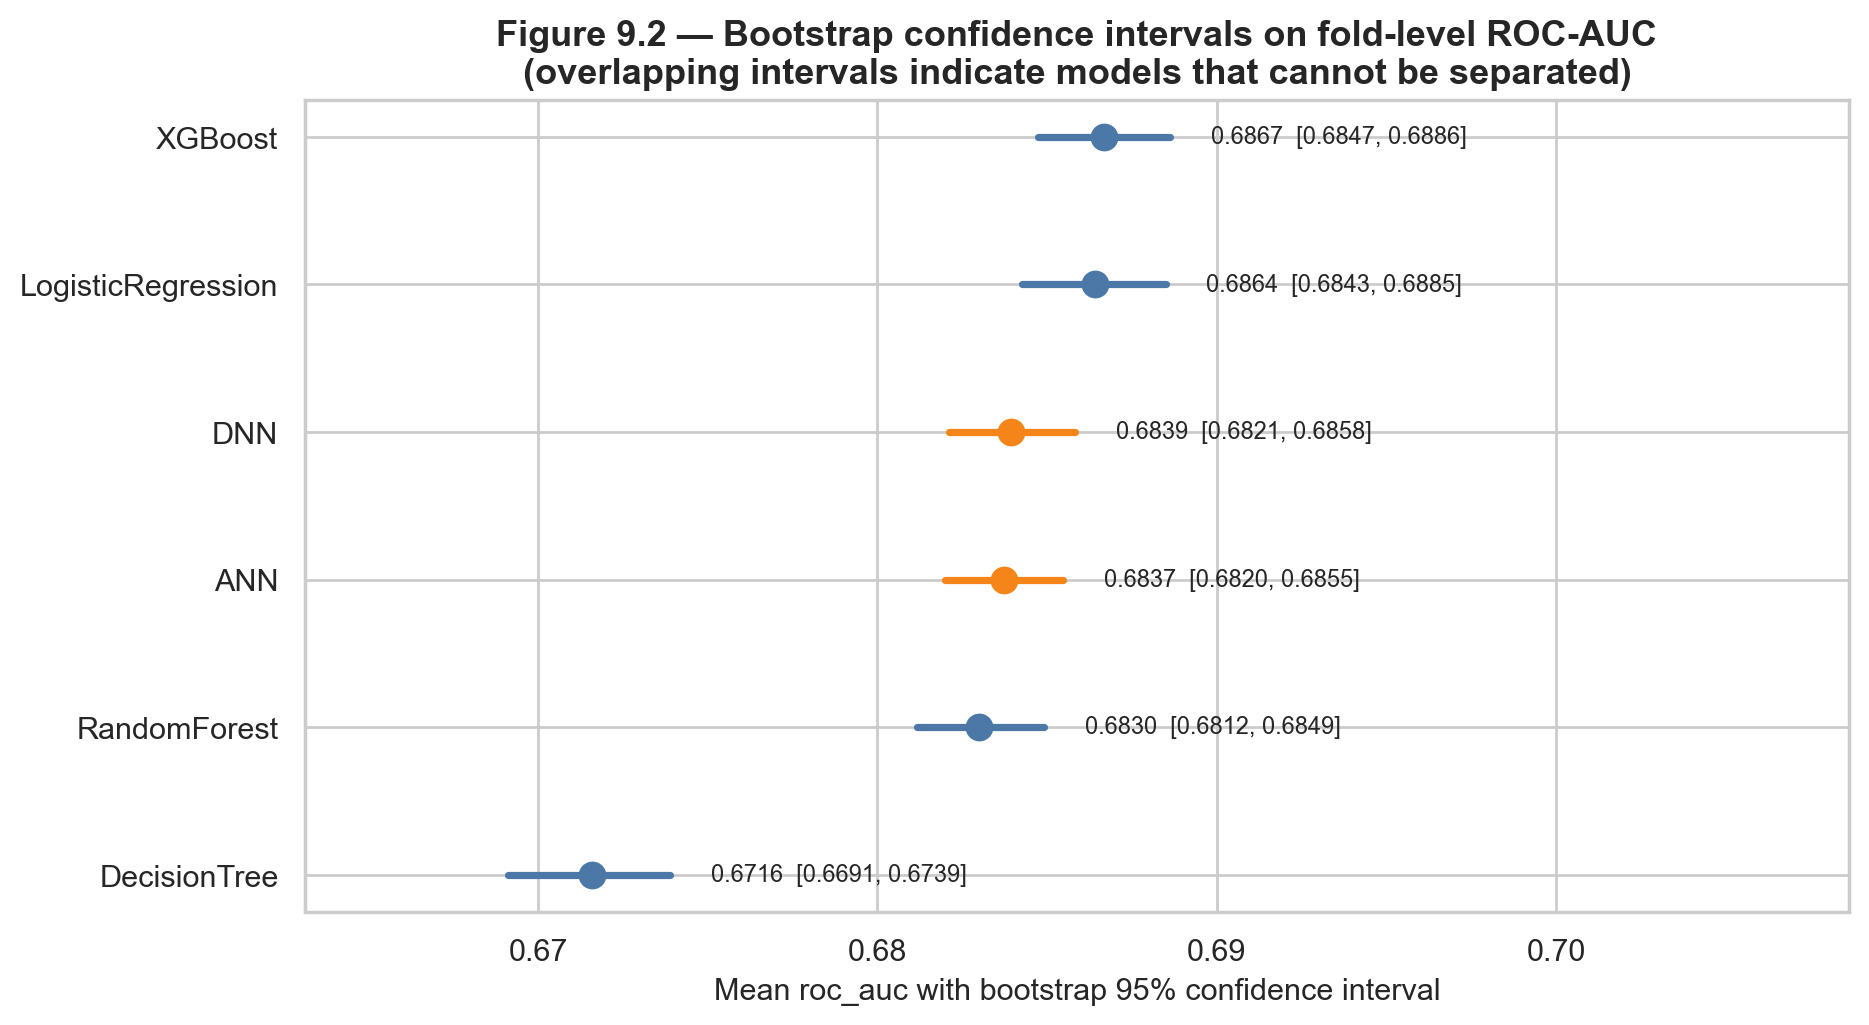
\includegraphics[width=\columnwidth]{fig_9_2_forest}
\caption{Mean ROC-AUC of the six finalists over $5\times3$ repeated cross-validation with bootstrap 95\% intervals (blue: ML; orange: DL).}
\label{fig:forest}
\end{figure}

The selection rule chose \ChampionLong{}: its tuned and engineered variants scored within one fold-level standard deviation of it (0.6875 against 0.6864) and it is the fastest of the three. Fig.~\ref{fig:forest} shows the six finalists under repeated cross-validation. Of the 15 pairwise comparisons, 12 are significant after Holm correction, but only 5 are material, and all five involve the decision tree. Seven comparisons are significant and negligible. Logistic regression and XGBoost cannot be separated (difference 0.0003, adjusted $p=0.36$), nor can the two networks ($p=0.62$). Logistic regression leads the ANN by 0.0027 and the DNN by 0.0025; these differences are highly consistent across folds ($d_z=-1.7$ and $-1.8$, adjusted $p<10^{-4}$) and are half the size we declared worth acting on. This is the case the materiality threshold exists for: with paired folds on 200,000 rows almost any difference becomes significant, and a study reporting only $p$-values would announce a ranking that has no practical content.

Training time, in contrast, separates the families both significantly and materially. In the same repeated folds the ANN took 55~s and the DNN 94~s longer per fit than logistic regression (bootstrap intervals 51--59~s and 82--107~s; adjusted $p<0.001$).

\subsection{Held-out test performance}
\begin{table}[t]
\caption{Performance on \NTest{} held-out customers after refitting on \NTrain{} rows. Cfg.: experiment whose configuration was used. $^{\dagger}$: selected model. Threshold-dependent metrics at each model's own F1-optimal cut-off}
\label{tab:test}
\centering
\footnotesize
\setlength{\tabcolsep}{3.5pt}
\begin{tabular}{@{}lccccccc@{}}
\toprule
Model & Cfg. & AUC & PR-AUC & F1 & Rec. & Prec. & Acc. \\
\midrule
% Generated by make_macros.py -- do not edit by hand.
ANN & B & 0.6851 & 0.2045 & 0.268 & 0.374 & 0.209 & 0.797 \\
DNN & B & 0.6849 & 0.2032 & 0.269 & 0.425 & 0.197 & 0.771 \\
LR$^{\dagger}$ & A & 0.6848 & 0.2031 & 0.269 & 0.444 & 0.193 & 0.760 \\
XGB & C & 0.6843 & 0.2053 & 0.269 & 0.452 & 0.191 & 0.755 \\
RF & C & 0.6794 & 0.1998 & 0.265 & 0.448 & 0.188 & 0.753 \\
DT & C & 0.6712 & 0.1849 & 0.257 & 0.441 & 0.181 & 0.747
\\
\bottomrule
\end{tabular}
\end{table}

Table~\ref{tab:test} reports the final evaluation. The six models span \TestSpread{} ROC-AUC, and the first four, two from each family, lie within 0.0008 of one another (0.6843--0.6851). The cross-validated estimate for the selected model was optimistic by only 0.0016, so the protocol did not overfit the development sample. The order within the leading group did change: on the test set the ANN is 0.0004 and the DNN 0.0001 ahead of logistic regression, where cross-validation had placed them 0.0025 behind. The reason is the amount of training data and not chance alone, since the finalists were refitted on four times as many rows and the networks were still improving with data at the size of the development sample (Section~\ref{sec:why}). We report this as it is: the selected model was not the top-scoring model on the test set, and the margin by which it was not is one-fourteenth of the materiality threshold. The four leading models also rank customers almost identically (pairwise Spearman correlation of test scores $\geq0.983$).

Two further points follow from Table~\ref{tab:test}. The F1-optimal thresholds lie between 0.12 and 0.15, far from 0.5, and at these thresholds every model has an accuracy of 0.75--0.80, below the 0.901 obtained by predicting that nobody churns. Accuracy, the metric reported by \LitAllAcc\% of the screened literature, would have ranked the useless majority classifier first. The differences in recall and precision between models in Table~\ref{tab:test} reflect where each threshold fell on a flat F1 curve; the F1 values themselves differ by less than 0.005 among the leading four.

\subsection{Execution cost}
\begin{table}[t]
\caption{Execution cost of the finalists. Train: full fit on \NTrain{} rows. Batch: per customer in a 20,000-row batch. Online: median single-request latency with 1 and with 8 concurrent workers; RPS: requests per second at 8 workers}
\label{tab:runtime}
\centering
\footnotesize
\setlength{\tabcolsep}{3pt}
\begin{tabular}{@{}llrrrrrr@{}}
\toprule
 & & Train & Epoch & Batch & \multicolumn{2}{c}{Online (ms)} & \\
\cmidrule(lr){6-7}
Model & Dev. & (s) & (s) & ($\mu$s) & 1 & 8 & RPS \\
\midrule
% Generated by make_macros.py -- do not edit by hand.
ANN & GPU & 191 & 10.9 & 4.0 & 5.5 & 43 & 184 \\
DNN & GPU & 305 & 27.3 & 5.0 & 10.4 & 83 & 95 \\
LR & CPU & 4 & -- & 1.2 & 2.0 & 2 & 550 \\
XGB & CPU & 10 & -- & 1.9 & 2.5 & 19 & 363 \\
RF & CPU & 94 & -- & 6.1 & 34.5 & 163 & 49 \\
DT & CPU & 15 & -- & 1.7 & 2.2 & 10 & 401
\\
\bottomrule
\end{tabular}
\end{table}

\begin{figure*}[t]
\centering
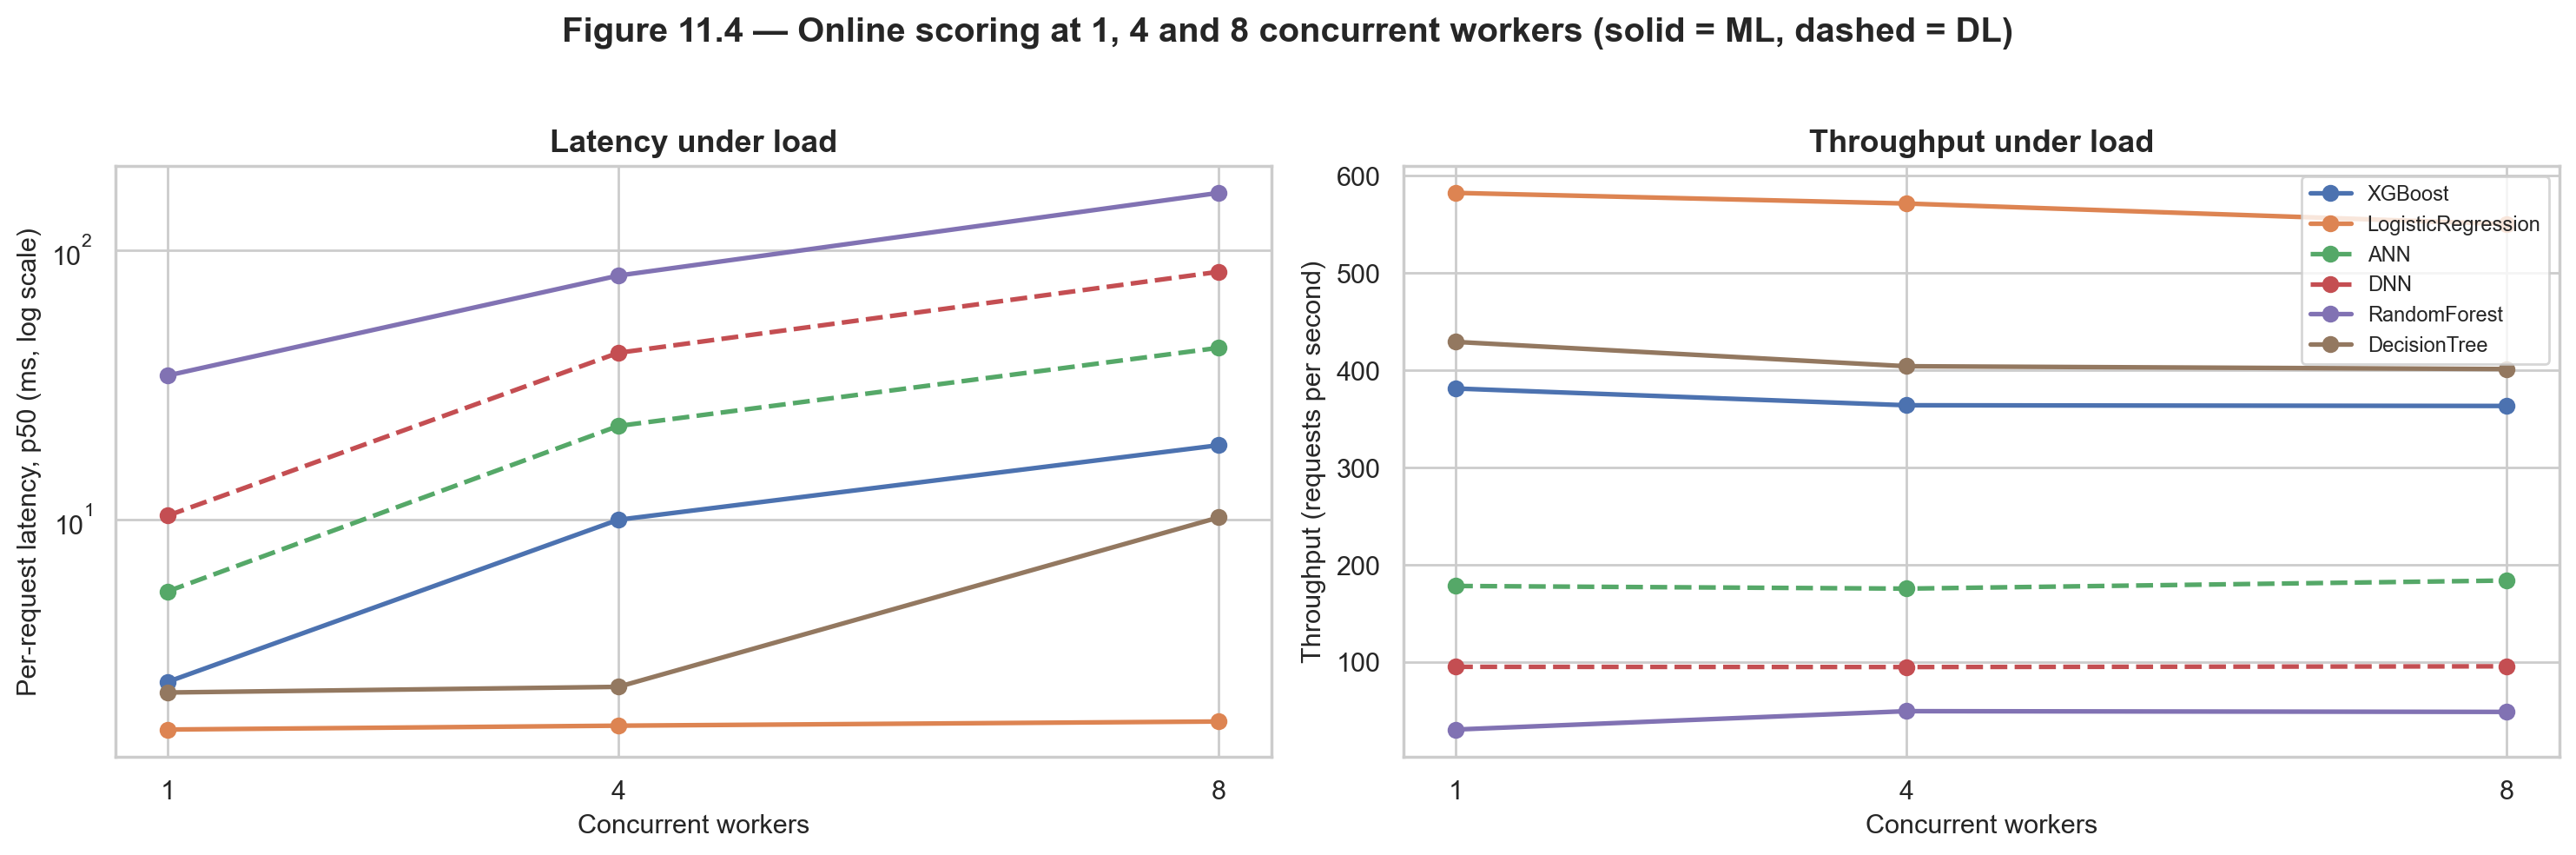
\includegraphics[width=0.9\textwidth]{fig_11_4_concurrency}
\caption{Median single-request latency and throughput with 1, 4 and 8 concurrent workers (solid: ML; dashed: DL).}
\label{fig:conc}
\end{figure*}

Table~\ref{tab:runtime} shows what the equal accuracy costs. Fitting logistic regression on \NTrain{} rows took 4~s and XGBoost 10~s; the ANN took 191~s (16 epochs at 10.9~s) and the DNN 305~s (10 epochs at 27.3~s), that is, \TrainRatioBestDl{} and 80 times longer than the selected model. A single request is answered in \ChampOnlineMs{}~ms by logistic regression, 2.5~ms by XGBoost, \BestDlOnlineMs{}~ms by the ANN and 10.4~ms by the DNN. The random forest is the slowest model online (34.5~ms), a reminder that latency is a property of the model and not of its family.

The gap widens under load (Fig.~\ref{fig:conc}). With eight concurrent workers logistic regression still answers in 1.8~ms and sustains 550 requests per second. The networks' throughput does not increase with the number of workers (178 to 184 requests per second for the ANN, 95 for the DNN) because requests queue for one accelerator, so their median latency grows in proportion to the queue, to 43~ms and 83~ms. A service-level objective of 50~ms at eight concurrent callers is met by the ANN with little margin and missed by the DNN, on a model whose test ROC-AUC equals that of logistic regression to three decimals.

\begin{table}[t]
\caption{The same networks on CPU and GPU (100,000 rows, six epochs, batch size 1,024)}
\label{tab:device}
\centering
\footnotesize
\begin{tabular}{@{}llccc@{}}
\toprule
Model & Device & Epoch (s) & Batch ($\mu$s) & Online (ms) \\
\midrule
% Generated by make_macros.py -- do not edit by hand.
ANN & CPU & 0.17 & 3.5 & 3.6 \\
ANN & GPU & 1.36 & 3.9 & 5.9 \\
DNN & CPU & 0.63 & 4.0 & 6.7 \\
DNN & GPU & 3.36 & 4.6 & 10.2
\\
\bottomrule
\end{tabular}
\end{table}

Table~\ref{tab:device} isolates the effect of the accelerator. On the GPU one epoch took \GpuSlowdownAnn{} times longer for the ANN and \GpuSlowdownDnn{} times longer for the DNN than on the CPU, and single-request latency was 1.5--1.6 times higher, with the same ROC-AUC after six epochs. Networks of this size on tabular input are dominated by the per-batch cost of dispatching work to the device and not by arithmetic, so there is nothing for the GPU to accelerate. The common assumption that deep learning's cost can be bought back with a GPU does not hold for tabular churn models of the size used in the literature. The network timings in Table~\ref{tab:runtime} are therefore upper bounds for this hardware: on the CPU the networks would train several times faster, which would still leave them an order of magnitude slower to train than logistic regression or XGBoost.

\subsection{Interpretability}
For the selected model SHAP values are exact and cost 0.007~ms per customer. Seven of its 38 encoded features carry 80\% of the total attribution; a two-year contract alone carries 34.8\%, followed by a one-year contract, satisfaction score, technical support, complaints, service calls and late payments. The negative control passed: the twelve uninformative features received 1.97\% of the attribution (0.06 times the share of an average feature) and a median rank of 24 of 38. The SHAP ranking agrees with the ranking from the exploratory analysis ($\rho=0.66$, $p<0.001$).

For the ANN no exact explainer exists. KernelSHAP took 312~ms per customer, four orders of magnitude more, and its estimates depend on the background sample and the number of coalitions. The ANN's ranking agrees only moderately with that of logistic regression ($\rho=0.51$; four of the ten leading features in common), although the two models' scores are nearly interchangeable ($\rho=0.985$). The network spreads its attribution over engineered composites, led by the contract-and-payment segment, where the linear model concentrates it on contract type. Two models that make the same decisions thus give different accounts of why. For a bank that must give customers and supervisors reasons for automated decisions, an exact, stable and nearly free explanation is a functional requirement, and it is available for one of these two models.

\subsection{Campaign value}
At a contact depth of \CampaignSharePct\% of one million customers, logistic regression captures 6,836 churners among the 20,000 contacted, the ANN 6,891 ($+0.8\%$) and the DNN 6,947 ($+1.6\%$). Under the assumed business parameters the mean net monthly value is \$467k, \$478k and \$490k respectively, inside a 5th--95th percentile range of $-$\$0.86M to \$2.7M that is governed by customer value, offer cost and save rate and is almost identical for the three models. On paired draws the ANN is ahead of logistic regression in 61\% and the DNN in 73\% of cases, with a mean advantage of \$11k and \$23k per month and 90\% intervals that include zero ($-$\$58k to $+$\$94k for the ANN).

Two conclusions follow, and the first runs against our own expectation. Compute cost does not decide the choice: the serving, rescoring and retraining bill is \$175 per month for logistic regression, \$263 for the ANN and \$526 for the DNN, and the networks' extra cost is repaid by fewer than two additional retained customers per month. An argument against deep learning that rests on the cloud bill is not supported by these data. Second, the networks' advantage in capture is small, uncertain and not specific to deep learning. On the test set the model that captured the most churners at every depth from 0.5\% to 5\% was tuned XGBoost (1,426 of 4,000 contacted at 2\% depth, against 1,373 for logistic regression), a model that trains in 10~s, answers in 2.5~ms and has an exact SHAP explainer. Logistic regression was not the best model at any of the six depths examined, which shows that selecting on whole-curve ROC-AUC does not guarantee the best top of the list; a bank with a fixed contact budget should select on capture at that budget.

\subsection{Does tuning the networks change the answer?}\label{sec:nettuneres}
\begin{table}[t]
\caption{The tuned network against the reference models. CV: mean ROC-AUC over the 15 repeated folds. Train: full fit on \NTrain{} rows (default networks on the GPU, tuned network on the CPU; range over three seeds). $^{\dagger}$: selected model}
\label{tab:dltune}
\centering
\footnotesize
\setlength{\tabcolsep}{3.5pt}
\begin{tabular}{@{}lcccc@{}}
\toprule
 & CV & Test & Train & Online \\
Model & AUC & AUC & (s) & (ms) \\
\midrule
% Generated by make_macros.py -- do not edit by hand.
LR$^{\dagger}$ & 0.6864 & 0.6848 & 4 & 2.0 \\
XGB (tuned) & 0.6867 & 0.6843 & 10 & 2.5 \\
ANN (default) & 0.6837 & 0.6851 & 191 & 5.5 \\
DNN (default) & 0.6839 & 0.6849 & 305 & 10.4 \\
Tuned network & 0.6866 & 0.6846--0.6847 & 34--52 & 5.2 \\
Tuned network, 3 seeds averaged & -- & 0.6854 & 121 & --
\\
\bottomrule
\end{tabular}
\end{table}

The default networks trailed logistic regression under cross-validation, and the obvious objection is that they were not tuned. We therefore tuned them (Section~\ref{sec:nettune}). The search took 36 minutes; 28 trials completed and 22 were pruned. It raised the cross-validated ROC-AUC on the tuning sample from 0.6813 and 0.6819 for the two default configurations to 0.6879.

The configuration it selected is informative in itself: four hidden layers of only 16 SELU units, no batch normalisation, dropout of 0.16, a light L2 penalty, the engineered features, and the direct linear path from inputs to output, 1,937 parameters in all and smaller than either default network. Nine of the ten best configurations used the linear path, none used batch normalisation and none used ReLU. Given freedom over depth, width and activation, the search moved the network towards logistic regression.

Table~\ref{tab:dltune} gives the outcome. On the 15 repeated folds the tuned network scored 0.6866 against 0.6864 for logistic regression, a difference of $+0.0002$ (bootstrap 95\% interval $-0.0002$ to $+0.0007$; paired $t$-test $p=0.36$), ahead in 10 folds and behind in 5. It is equally indistinguishable from tuned XGBoost ($-0.00004$, $p=0.85$). Tuning did help the network: it beat the default ANN and DNN in all 15 folds, by 0.0029 and 0.0027 ($p<10^{-5}$), which removes the networks' cross-validation deficit entirely, although the gain is itself below the materiality threshold. On the test set the three seeds scored between 0.6846 and 0.6847 against 0.6848 for logistic regression (paired bootstrap 95\% interval for the difference $-0.0009$ to $+0.0005$), and no higher than the default ANN refitted on the full training partition (0.6851). Averaging the three seeds gave 0.6854, which is 0.0006 above logistic regression at three times the training cost; at a 2\% contact depth it captured 1,384 churners against 1,373 for logistic regression, 1,367 for a single tuned network and 1,426 for XGBoost.

The tuned network is cheaper than the default ones but not cheap: it trained in 34--52~s on the CPU, 9--14 times longer than logistic regression, before counting the search, and answered a single request in 5.2~ms against 2.0~ms. The result is therefore stated plainly: with a fair tuning budget the best network we could build equals logistic regression and tuned XGBoost on these data and does not beat them.

\subsection{Why capacity does not pay on these data}\label{sec:why}
\begin{figure}[t]
\centering
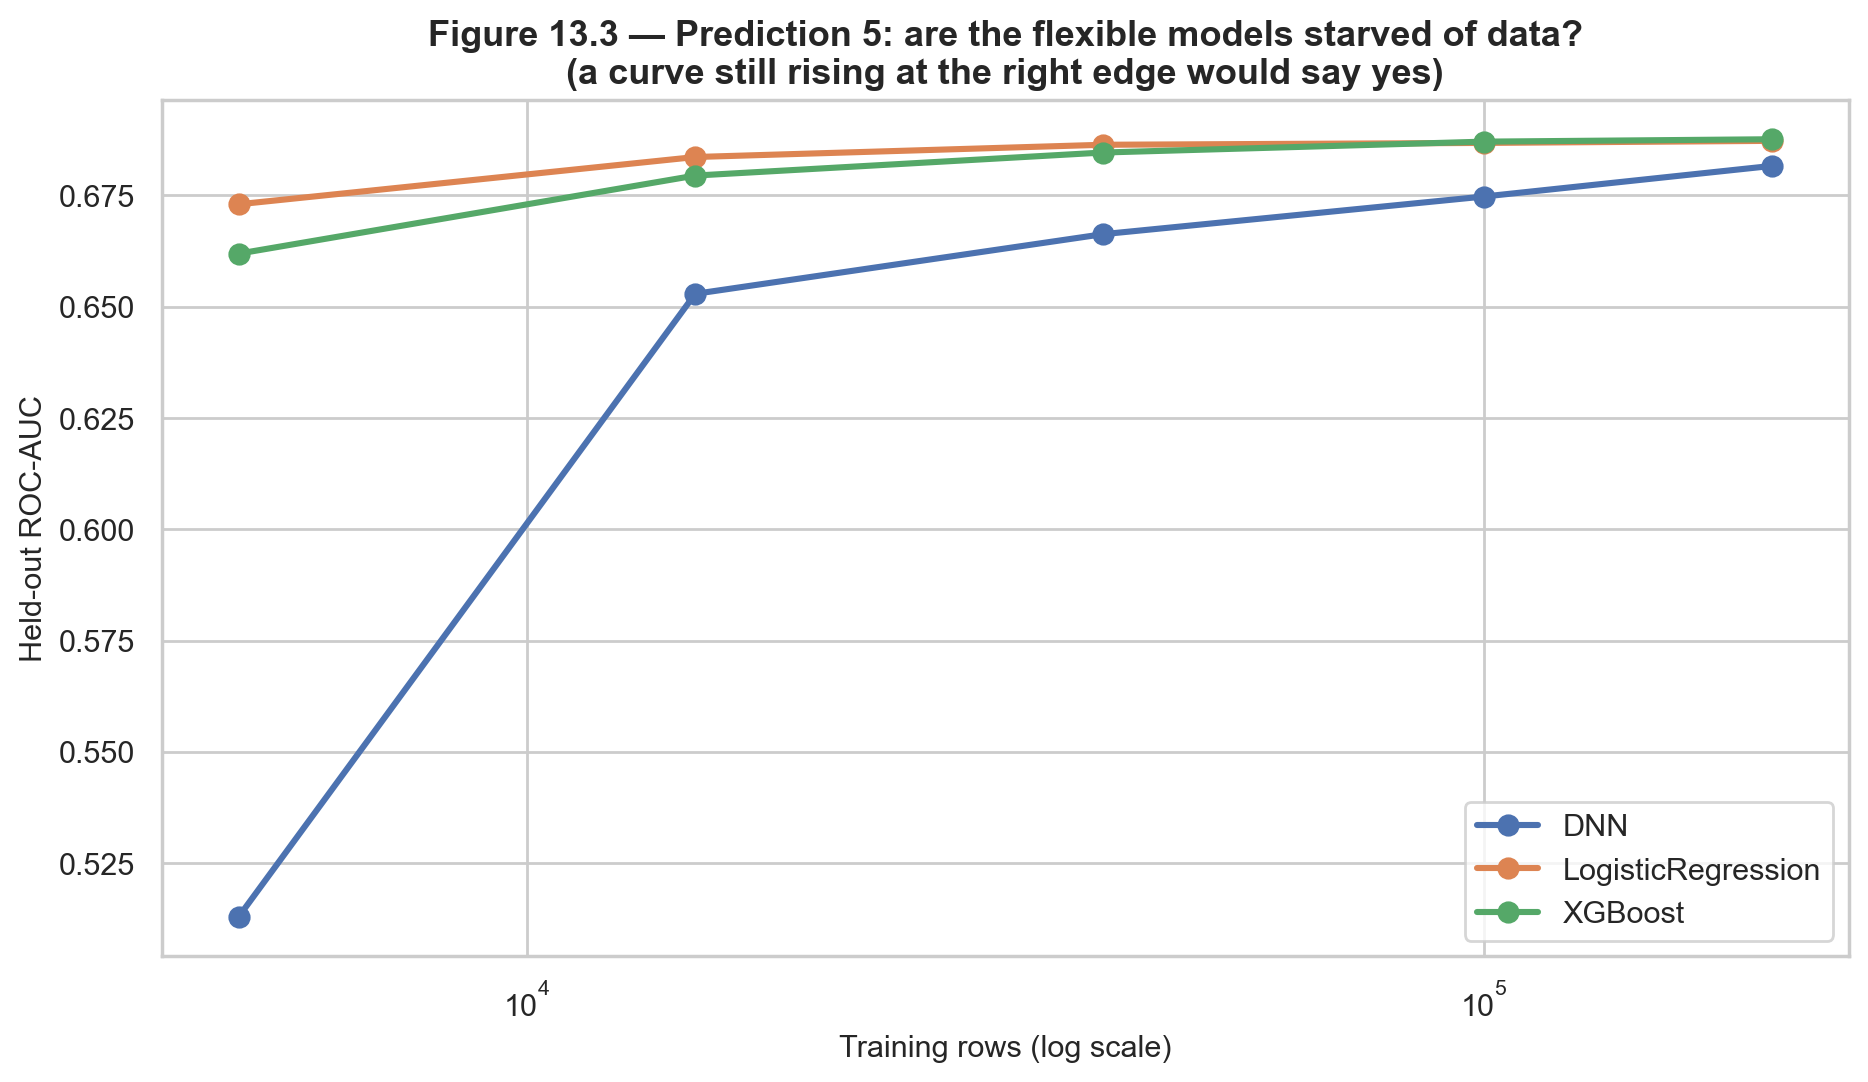
\includegraphics[width=\columnwidth]{fig_13_3_learning_curves}
\caption{Held-out ROC-AUC against the number of training rows.}
\label{fig:lc}
\end{figure}

All six predictions of the additive-linear hypothesis were supported. (1) The empirical log-odds of churn are linear in the main drivers (mean $R^2=0.95$). (2) Adding cubic splines to logistic regression changes ROC-AUC by $+0.0005$ and (3) adding all pairwise interactions by $-0.0006$, both well inside one fold-level standard deviation (0.003). (4) The flexible models reproduce the linear model's ranking (minimum Spearman correlation 0.96; 85\% overlap in the customers selected for the campaign). (5) With more data the flexible models converge on the linear model and do not pass it materially (Fig.~\ref{fig:lc}): from 5,000 to 200,000 rows logistic regression gains 0.014, XGBoost exceeds it by at most 0.0004, and the DNN climbs from 0.513 to 0.682, still rising by 0.007 over the last doubling and 0.006 short. (6) The strongest single feature reaches a ROC-AUC of only 0.61 and the best model 0.685, so the ceiling is a property of the signal.

A network earns its capacity by finding interactions and non-linearities that simpler models miss. Tests (2) and (3) show that there are none of material size to find here, and test (5) shows what the network pays to discover that: it needs more than ten times as many rows as logistic regression to reach the same ROC-AUC (the DNN at 200,000 rows scores what logistic regression scores at about 15,000). The tuning study (Section~\ref{sec:nettuneres}) reaches the same conclusion from the other side: a search free to add depth, width and non-linearity chose a small network with a direct linear path, and that network arrived at the ceiling shared by logistic regression, splines, interactions and boosted trees and went no further.

\subsection{Should deep learning always be used in production?}
On the evidence of this study, no. The reason is not that the networks were less accurate, since at full data volume, and after tuning at any data volume, they were not, nor that they were expensive to run, since at cloud prices they were not. It is that they offered no material gain to set against four costs that a simple model does not incur: a training time 50--80 times longer at literature settings and 9--14 times longer after a tuning search that is itself an added cost, which lengthens every retraining and every experiment; a latency three to five times higher that degrades further under concurrency; a need for far more data to reach the same accuracy, which matters for a new product or a small portfolio; and explanations that are approximate, costly and inconsistent with those of an equally accurate transparent model. This agrees with benchmark evidence that deep models do not dominate tree ensembles on tabular data~\cite{grinsztajn2022tree,shwartzziv2022tabular,borisov2024deep}, and it extends that evidence from accuracy to the operational properties on which a deployment decision turns.

The answer is conditional, and the condition can be tested cheaply before any network is built. If splines or pairwise interactions added to a logistic regression produce a material gain, or if boosted trees materially outperform the linear model, the signal contains structure that capacity can exploit and a network becomes a candidate; the same holds where the inputs are sequences of transactions or text, to which the architectures reported as superior in the banking literature~\cite{haddadi2022iranian,latheef2021lstm} are suited and ours are not. Where these checks are negative, as here, the defensible production choice is a tuned gradient-boosted ensemble or a regularised linear model.

% =============================================================================
\section{Conclusion}
% =============================================================================
We compared four machine-learning models, two deep-learning models at literature settings and one tuned network for churn prediction on one million customers under a single leakage-controlled protocol. The two families were statistically separable and practically equivalent: the four leading models lay within 0.0008 ROC-AUC on \NTest{} held-out customers, and differences of 0.003 under cross-validation were highly significant and immaterial. What separated them was everything other than accuracy. Tuning the network over depth, width, activation and regularisation removed its small cross-validation deficit and produced a model indistinguishable from logistic regression and XGBoost, not a better one. The networks took 9--14 times longer to train after tuning and 50--80 times longer at literature settings, answered three to five times more slowly, lost throughput under concurrent load, needed more than ten times as much data to match a linear model, were several times slower on a GPU than on a CPU, and could be explained only approximately. A six-part diagnosis traced the equivalence to the data: the log-odds of churn are linear and additive in the available features, so additional capacity has nothing to learn.

The study also measured how much of a reported result can be produced by method. Oversampling before splitting inflated ROC-AUC by 0.32; default tree ensembles understated their tuned versions by 0.015; imbalance treatments moved recall by 0.37 and ROC-AUC by 0.02; and accuracy ranked a classifier that identifies no churner above every model. Each of these effects exceeds the difference between the model families, which is reason to read single-protocol claims of deep-learning superiority in the churn literature with caution.

For practitioners we recommend the following order of work: fix a leakage-safe pipeline; fit a regularised linear model and a tuned boosted ensemble; test for non-additive structure with splines and interactions; and consider a network only if that test is positive, evaluating it on capture at the campaign's contact depth, on latency under the expected concurrency, and on the explanation it can give.

The limitations are these. The results come from one dataset with a subscription-service schema that shows signs of simulation, so the numerical values do not transfer to a particular bank, although the protocol does. The networks are feed-forward. The tuned network received a single 50-trial search, and the interpretability, concurrency and campaign analyses were run on the default networks and not repeated for it; attention-based tabular architectures~\cite{pasaribu2024tabular} and sequence models on transaction histories were not evaluated. Timings come from one machine with an integrated GPU, and a discrete accelerator with larger batches may behave differently. The business parameters of the simulation are assumptions. Future work should repeat the protocol on institutional banking data with transaction sequences, add attention-based networks to the comparison, and replace campaign capture with measured uplift from a controlled retention experiment.

\bibliographystyle{IEEEtran}
\bibliography{references}

\end{document}
